\documentclass[12pt]{article}
\usepackage{setspace}
\usepackage{geometry}
\usepackage{adjustbox}
\geometry{verbose,lmargin=2cm,rmargin=2cm,bmargin=2.5cm,tmargin=2cm}

\usepackage{booktabs}
\usepackage{natbib}
\usepackage{hyperref}
\hypersetup{colorlinks=true,linkcolor=blue,urlcolor=blue}



\newcommand{\rootdir}{..}  % one dir up
\newcommand{\plots}{\rootdir/output/plots}
\newcommand{\tables}{\rootdir/output/tables}


%% TITLE PAGE
\begin{document}
\onehalfspacing
    
    
\title{A Reproducible Benchmark of Fixed Effects Estimation}



\author{Florian Oswald\thanks{RES Data Editor. You can find the source code generating the entire workshop at \url{https://github.com/floswald/ReproData.jl}}}
\date{\today}


\maketitle
\begin{abstract}
We illustrate a workflow which tries to address several pitfalls when creating a reproducible research project. We focus on preserving raw data, documenting data sources, creating a folder structure, writing stata and R code in a way which helps to preserve the package version environment, outputting results to disk and referencing them in a final output document. As a by-product, we report timings of a typical two-way fixed effects estimation exercise on a large dataset.    
\end{abstract}

\section{Introduction}

One could be forgiven to think that reproducibility is as simple as following a few simple steps:

\begin{enumerate}
\item Preserve raw data
\item Document data origin
\item Preserve code and document how to use it
\item Run everything again before submitting the package.
\end{enumerate}

While this is a good start, this list if far from exhaustive, and a more complete version is available under \url{https://datacodestandard.org}. Whatever the list, however, the devil is in the details, and \emph{in practice} achieving reproducibility is far from trivial. We want to use this fictitious research project to illustrate one potential strategy when setting up code, and data, and a few associated pitfalls. 

\section{Computational Task}

In this paper, we want to estimate the following linear regression with two fixed effects:

\begin{equation}
y_{ij} = \beta X_{ij} + \alpha_i + \gamma_j + u_{ij} \label{eq:1}
\end{equation}
where $X_{ij}$ is a matrix which stacks the 1 by 7 vectors $[ x_{ij1}, \dots, x_{ij7}]$. The indices $(i,j)$ group observations along two ad-hoc dimensions: imagine person and time, or worker and firm specific effects. Those $\alpha_i,\gamma_j$ are unobservable.

We generated the data such that the first $x$ is a function of both fixed effects, $x_{it1} = g(\alpha_i, \gamma_t)$, the second a function only of $\gamma_t$, $x_{it2} = h(\gamma_t)$, and we set the true values for coefficients to $\beta = [ 3,3,1,1,1,1,1]$. Now let me show you the first result in table \ref{tab:1}. Observe that models (1) and (2) exhibit bias, and only after we account for both fixed effects, we get the correct results. Overall this seems to work.\footnote{The interested reader may consult the data generating process \href{https://github.com/floswald/ReproData.jl/blob/main/src/ReproData.jl}{here}.}

\begin{table}
\centering
{
\def\sym#1{\ifmmode^{#1}\else\(^{#1}\)\fi}
\begin{tabular}{l*{4}{c}}
\toprule
                    &\multicolumn{1}{c}{(1)}&\multicolumn{1}{c}{(2)}&\multicolumn{1}{c}{(3)}&\multicolumn{1}{c}{(4)}\\
                    &\multicolumn{1}{c}{y}&\multicolumn{1}{c}{y}&\multicolumn{1}{c}{y}&\multicolumn{1}{c}{y}\\
\midrule
x1                  &       3.982\sym{***}&       3.494\sym{***}&       3.001\sym{***}&       2.998\sym{***}\\
                    &   (0.00108)         &   (0.00553)         &   (0.00778)         &   (0.00318)         \\
\addlinespace
x2                  &       3.019\sym{***}&       3.497\sym{***}&       3.003\sym{***}&       3.001\sym{***}\\
                    &   (0.00151)         &   (0.00553)         &   (0.00779)         &   (0.00318)         \\
\addlinespace
x3                  &                     &                     &                     &       1.000\sym{***}\\
                    &                     &                     &                     &  (0.000318)         \\
\addlinespace
x4                  &                     &                     &                     &       1.000\sym{***}\\
                    &                     &                     &                     &  (0.000318)         \\
\addlinespace
x5                  &                     &                     &                     &       1.001\sym{***}\\
                    &                     &                     &                     &  (0.000318)         \\
\addlinespace
x6                  &                     &                     &                     &       1.000\sym{***}\\
                    &                     &                     &                     &  (0.000318)         \\
\addlinespace
x7                  &                     &                     &                     &       1.000\sym{***}\\
                    &                     &                     &                     &  (0.000318)         \\
\addlinespace
Constant            &     0.00114         &    0.000955         &   -0.000234         &    -0.00164\sym{***}\\
                    &  (0.000775)         &  (0.000775)         &  (0.000775)         &  (0.000316)         \\
\midrule
FE 1                &          No         &         Yes         &         Yes         &         Yes         \\
FE 2                &                     &                     &                     &                     \\
Observations        &    10000000         &    10000000         &    10000000         &    10000000         \\
\bottomrule
\multicolumn{5}{l}{\footnotesize Standard errors in parentheses}\\
\multicolumn{5}{l}{\footnotesize \sym{*} \(p<0.10\), \sym{**} \(p<0.05\), \sym{***} \(p<0.01\)}\\
\end{tabular}
}

\caption{This is done with stata. I couldn't figure out why the FE2 row does not display a "yes" in columns 3 and 4. My bad, sorry!\label{tab:1}}
\end{table}
Let us also have a table produced by R. We show the results in table \ref{tab:2} and in figure \ref{fig:1}.

\begin{table}
\centering

\begingroup
\centering
\begin{tabular}{lcccc}
   \tabularnewline \midrule \midrule
   Dependent Variable: & \multicolumn{4}{c}{y}\\
   Model:       & (1)           & (2)           & (3)           & (4)\\  
   \midrule
   \emph{Variables}\\
   Constant     & 0.0011        &               &               &   \\   
                & (0.0008)      &               &               &   \\   
   x1           & 3.982$^{***}$ & 3.494$^{***}$ & 3.001$^{***}$ & 2.998$^{***}$\\   
                & (0.0011)      & (0.0055)      & (0.0078)      & (0.0032)\\   
   x2           & 3.019$^{***}$ & 3.497$^{***}$ & 3.003$^{***}$ & 3.001$^{***}$\\   
                & (0.0015)      & (0.0055)      & (0.0078)      & (0.0032)\\   
   x3           &               &               &               & 0.9996$^{***}$\\   
                &               &               &               & (0.0003)\\   
   x4           &               &               &               & 0.9998$^{***}$\\   
                &               &               &               & (0.0003)\\   
   x5           &               &               &               & 1.001$^{***}$\\   
                &               &               &               & (0.0003)\\   
   x6           &               &               &               & 1.000$^{***}$\\   
                &               &               &               & (0.0003)\\   
   x7           &               &               &               & 1.000$^{***}$\\   
                &               &               &               & (0.0003)\\   
   \midrule
   \emph{Fixed-effects}\\
   id1          &               & Yes           & Yes           & Yes\\  
   id2          &               &               & Yes           & Yes\\  
   \midrule
   \emph{Fit statistics}\\
   Observations & 10,000,000    & 10,000,000    & 10,000,000    & 10,000,000\\  
   R$^2$        & 0.84518       & 0.84685       & 0.84698       & 0.97449\\  
   Within R$^2$ &               & 0.80515       & 0.02917       & 0.83816\\  
   \midrule \midrule
   \multicolumn{5}{l}{\emph{Signif. Codes: ***: 0.01, **: 0.05, *: 0.1}}\\
\end{tabular}
\par\endgroup



\caption{This is done with R.\label{tab:2}}
\end{table}

\begin{figure}
\centering
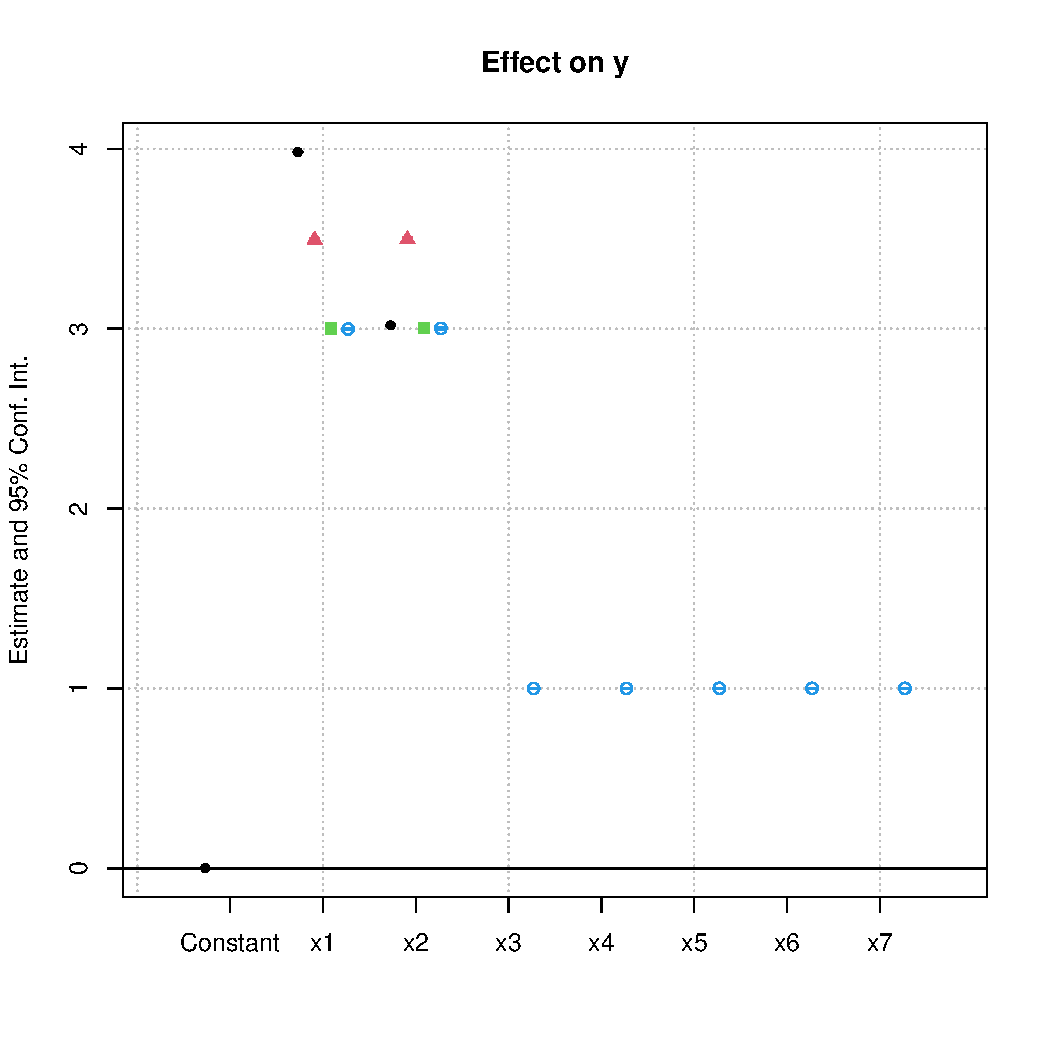
\includegraphics[width=0.8\textwidth]{\plots/figure1.pdf}
\caption{The coef plot corresponding to table \ref{tab:2}\label{fig:1}.}
\end{figure}

\section{Timings}

We found that this leads to the following result in terms of run time between stata and R, which are displayed in table \ref{tab:3}.

\begin{table}[]
\centering
\begin{tabular}{lcc}
\toprule
    Operation & Stata & R  \\
    \midrule
    CSV read & 62.43 & 1.493  \\
    FE estimation & 85.68 & 5.5  \\
    \bottomrule
\end{tabular}
\caption{Timing of operations in different languages in seconds.\label{tab:3}}
\end{table}
%%% note to replicators: those values are displayed on the console
%%% when running:
%%% `code/stata/run.do` and `code/R/script.R`
\nocite{*}

\newpage

\bibliography{grateful-refs}
\bibliographystyle{plainnat}

\end{document}
